% ============================================================
% CHƯƠNG 3 — THIẾT KẾ HỆ THỐNG
% Viết lại ngày 17/11/2026 theo yêu cầu của sinh viên: Chương 3 "Thiết kế, triển khai và đánh giá" đổi thành
% "Thiết kế hệ thống". Phần Xây dựng ứng dụng, Kiểm thử, Triển khai (cùng các bảng \BangCongNghe, \BangTest...,
% \HinhTrienKhai, \HinhCauTrucMa) chuyển sang Chap4.tex "Công nghệ, xây dựng và kiểm thử hệ thống".
% Bản trước: backup/2026-11-17_truoc-phantich-thietke/Chap3.tex.
%
% Bố cục theo mẫu SoICT: Thiết kế kiến trúc (lựa chọn kiến trúc, thiết kế tổng quan = biểu đồ gói,
% thiết kế chi tiết gói) -> Thiết kế chi tiết (giao diện, lớp, trình tự, API, CSDL).
% Đã thống nhất (07/11/2026): VVB chỉ phê duyệt, cơ quan quản lý phát hành (ISSUER_ROLE).
% [CẦN SỬA MÃ] contracts/contracts/CarbonCreditNFT.sol vẫn để mintBatch dưới VERIFIER_ROLE, trường
% CreditBatch.verifier (thiết kế: issuer), frontend/app/admin cấp VERIFIER_ROLE, nút mint ở /verifier.
% Các chương 4–6 chưa \input trong main.tex, nên chương này không \ref tới nhãn của các chương đó.
% Văn phong: xem ghi chú đầu Chap1.tex. [BẢN NHÁP] Sinh viên đọc lại và sửa theo văn phong của mình.
% ============================================================

\chapter{THIẾT KẾ HỆ THỐNG}
\label{chap:thietke}
% ============================================================
% HÌNH VẼ CHƯƠNG 3 — THIẾT KẾ HỆ THỐNG (TikZ), gọi bằng macro trong Chap3.tex
%   \HinhGoi         : biểu đồ gói (thiết kế tổng quan)     (fig:goi)        [thêm 17/11/2026]
%   \HinhOnOffChain  : phân tách dữ liệu on/off-chain       (fig:onoffchain)
%   \HinhTrangThai   : biểu đồ trạng thái của lô tín chỉ    (fig:trangthai)
% Đây là bản đề xuất theo phiếu giao nhiệm vụ: sửa lại cho khớp thiết kế thực tế của bạn.
% ============================================================

% Biểu đồ use case tổng quát (\HinhUseCase) và hình tác nhân (pic tacnhan) đã chuyển sang
% figures_chap2.tex ngày 17/11/2026, khi Chương 2 đổi thành "Phân tích hệ thống".

% ---------- Biểu đồ gói (thiết kế tổng quan) ----------
% Gói UML: thân gói (goi) và nhãn tên gói đặt ở góc trên bên trái (thẻ gói).
\tikzset{
  goi/.style={draw, fill=white, align=left, font=\scriptsize, inner sep=3pt, text width=#1},
  goi/.default=3cm,
  thegoi/.style={draw, fill=gray!15, font=\scriptsize\bfseries, inner sep=2pt, anchor=south west},
  phuthuoc/.style={->, >={Stealth[open]}, dashed},
  tang/.style={draw, thick, dashed, rounded corners=4pt, inner sep=7pt}
}
\newcommand{\HinhGoi}{%
\begin{figure}[htbp]
\centering
\begin{adjustbox}{max width=\textwidth}
\begin{tikzpicture}[nhan/.style={font=\scriptsize, fill=white, inner sep=1pt, align=center}]
  % Tầng giao diện
  \node[goi=3.4cm] (app) at (-4.3,3.9) {trang dự án, tra cứu, chứng nhận hủy,\\ dự án của tôi, thẩm định,\\ ví tín chỉ, dashboard, quản trị};
  \node[thegoi] (tapp) at (app.north west) {app};
  \node[goi=2.5cm] (comp) at (-0.2,3.9) {Nav, WalletProvider,\\ ui (ActionButton, Status)};
  \node[thegoi] at (comp.north west) {components};
  \node[goi=2.7cm] (lib) at (3.8,3.9) {api.js (gọi API REST)\\ chain.js (ethers.js)\\ contracts.json (ABI)};
  \node[thegoi] at (lib.north west) {lib};
  \coordinate (fetop) at ([yshift=4.5mm]tapp.north west);
  \node[tang, fit=(app)(comp)(lib)(fetop),
        label={[font=\scriptsize\bfseries, anchor=north west]north west:frontend (Next.js)}] (fe) {};
  % Tầng dịch vụ off-chain
  \node[goi=3.3cm] (routes) at (-4.6,-0.5) {auth, users, projects,\\ documents, issuance,\\ registry, dashboard, cadtrust};
  \node[thegoi] (troutes) at (routes.north west) {routes};
  \node[goi=2.6cm] (core) at (-0.8,-0.5) {auth.js (JWT, chữ ký ví)\\ validate.js, errors.js};
  \node[thegoi] at (core.north west) {core};
  \node[goi=3.3cm] (db) at (-4.6,-2.9) {db.js (truy vấn)\\ schema.sql (PostgreSQL)};
  \node[thegoi] at (db.north west) {db};
  \node[goi=2.6cm] (idx) at (-0.8,-2.9) {indexer.js\\ (đồng bộ sự kiện)};
  \node[thegoi] at (idx.north west) {indexer};
  \coordinate (betop) at ([yshift=4.5mm]troutes.north west);
  \node[tang, fit=(routes)(core)(db)(idx)(betop),
        label={[font=\scriptsize\bfseries, anchor=north west]north west:backend (Node.js, Express)}] (be) {};
  % Tầng on-chain
  \node[goi=2.1cm] (nft) at (3.6,-0.5) {ERC-721, lô tín chỉ,\\ chứng nhận hủy};
  \node[thegoi] (tnft) at (nft.north west) {CarbonCreditNFT};
  \node[goi=2.1cm] (pool) at (6.6,-0.5) {ERC-20 PCC,\\ NFT bị khóa};
  \node[thegoi] at (pool.north west) {CarbonPool};
  \node[goi=2.6cm] (oz) at (5.1,-2.9) {ERC721, ERC20,\\ AccessControl, Pausable,\\ ReentrancyGuard};
  \node[thegoi] at (oz.north west) {OpenZeppelin};
  \coordinate (sctop) at ([yshift=4.5mm]tnft.north west);
  \node[tang, fit=(nft)(pool)(oz)(sctop),
        label={[font=\scriptsize\bfseries, anchor=north west]north west:contracts (Solidity, Sepolia)}] (sc) {};
  % Phụ thuộc
  \draw[phuthuoc] (app) -- (comp);
  \draw[phuthuoc] (comp) -- (lib);
  \draw[phuthuoc] ([xshift=-6mm]lib.south) -- ++(0,-0.55) -| node[nhan, pos=0.25] {HTTP, JSON} (be.north);
  \draw[phuthuoc] ([xshift=8mm]lib.south) -- node[nhan] {JSON-RPC\\ qua MetaMask} ([xshift=8mm]lib.south |- sc.north);
  \draw[phuthuoc] (routes) -- (core);
  \draw[phuthuoc] (routes) -- (db);
  \draw[phuthuoc] (idx) -- (db);
  \draw[phuthuoc] (idx.east) -- node[nhan] {đọc sự kiện} (idx.east -| sc.west);
  \draw[phuthuoc] (pool) -- (nft);
  \draw[phuthuoc] (nft) -- (oz);
  \draw[phuthuoc] (pool) -- (oz);
\end{tikzpicture}
\end{adjustbox}
\caption[Biểu đồ gói của hệ thống]{Biểu đồ gói của hệ thống \hinhtao[Claude]{17/11/2026}}
\label{fig:goi}
\end{figure}}

% ---------- Phân tách dữ liệu on-chain / off-chain ----------
\newcommand{\HinhOnOffChain}{%
\begin{figure}[htbp]
\centering
\begin{tikzpicture}[
    >=Stealth,
    o/.style={draw, rounded corners=2pt, align=left, font=\footnotesize,
              text width=4.7cm, inner sep=4pt, fill=white},
    nhan/.style={font=\scriptsize, align=center, text width=2.6cm}]
  % Off-chain
  \node[o] (files) at (2.6,1.6) {\textbf{Kho tệp}\\
      thư mục lưu trữ của backend\\ (IPFS là hướng mở rộng):\\
      PDD, báo cáo giám sát,\\ báo cáo thẩm định};
  \node[o, below=5mm of files] (db) {\textbf{CSDL quan hệ}\\
      PostgreSQL, theo mô hình\\ CAD Trust V2.0:\\
      Project, Stakeholders,\\ Verifications, Issuances, Units;\\
      tài khoản ứng dụng (bảng riêng);\\
      lịch sử giao dịch đồng bộ từ sự kiện};
  \node[draw, thick, dashed, rounded corners=4pt, inner sep=6pt, fit=(files)(db),
        label={[font=\footnotesize\bfseries]above:Off-chain (backend)}] (off) {};
  % On-chain
  \node[o, fill=gray!10] (nft) at (11.0,1.6) {\textbf{Hợp đồng NFT tín chỉ (ERC-721)}\\
      tokenId, chủ sở hữu, số sê-ri,\\ mã băm hồ sơ, URI metadata};
  \node[o, fill=gray!10, below=4mm of nft] (pool) {\textbf{Hợp đồng pool (ERC-20)}\\
      số dư token,\\ NFT đang khóa trong pool};
  \node[o, fill=gray!10, below=4mm of pool] (ret) {\textbf{Chứng nhận hủy (trong hợp đồng NFT)}\\
      dãy sê-ri đã hủy, người hủy,\\ người thụ hưởng, sự kiện CreditRetired};
  \node[draw, thick, rounded corners=4pt, inner sep=6pt, fit=(nft)(pool)(ret),
        label={[font=\footnotesize\bfseries]above:On-chain (Ethereum Sepolia)}] (on) {};
  % Luồng dữ liệu
  \draw[->, thick] (files.east) -- node[nhan, above] {mã băm hồ sơ (keccak256) và URI khi mint}
      (on.west |- files.east);
  \draw[->, thick] (on.west |- db.east) -- node[nhan, below] {sự kiện CreditMinted, Transfer, CreditRetired: backend đồng bộ}
      (db.east);
\end{tikzpicture}
\caption[Phân tách dữ liệu giữa phần on-chain và off-chain của hệ thống]{Phân tách dữ liệu giữa phần on-chain và off-chain của hệ thống \hinhtao[Claude]{20/10/2026; Updated: 17/11/2026}}
\label{fig:onoffchain}
\end{figure}}

% ---------- Biểu đồ trạng thái của một lô tín chỉ ----------
\newcommand{\HinhTrangThai}{%
\begin{figure}[htbp]
\centering
\begin{tikzpicture}[
    >=Stealth,
    tt/.style={draw, rounded corners=6pt, align=center, font=\footnotesize,
               minimum height=0.9cm, inner xsep=5pt, fill=white},
    nhan/.style={font=\scriptsize, align=center}]
  \node[circle, fill=black, inner sep=3pt] (bd) at (0,0) {};
  \node[tt] (nhap)   at (1.4,0)   {Nháp};
  \node[tt] (cho)    at (4.5,0)   {Chờ thẩm định};
  \node[tt] (tuchoi) at (4.5,-2.3) {Bị từ chối};
  \node[tt] (dacap)  at (9.0,0)   {Đã cấp\\(NFT ERC-721)};
  \node[tt] (pool)   at (9.0,-2.6) {Trong pool\\(ERC-20)};
  \node[tt] (dahuy)  at (12.6,0)   {Đã hủy\\(retired)};
  \node[circle, draw, inner sep=4pt] (kt) at (14.1,0) {};
  \node[circle, fill=black, inner sep=2pt] at (kt) {};

  \draw[->] (bd) -- (nhap);
  \draw[->] (nhap) -- node[nhan, above] {gửi\\hồ sơ} (cho);
  \draw[->] (cho) -- node[nhan, above] {VVB duyệt; cơ quan\\quản lý mint NFT} (dacap);
  \draw[->] (cho) -- node[nhan, right] {VVB từ chối} (tuchoi);
  \draw[->] (tuchoi.west) -| node[nhan, pos=0.3, below] {bổ sung hồ sơ} (nhap.south);
  \draw[->] (dacap) -- node[nhan, above] {hủy hết\\(burn NFT)} (dahuy);
  \draw[->] (dahuy) -- (kt);
  \draw[->] ([xshift=-5mm]dacap.south) -- node[nhan, left] {nạp vào pool} ([xshift=-5mm]pool.north);
  \draw[->] ([xshift=5mm]pool.north) -- node[nhan, right] {đổi lại\\(redeem)} ([xshift=5mm]dacap.south);
  \draw[->] (pool.east) -| node[nhan, pos=0.3, below] {hủy hết phần còn lại\\ từ pool} (dahuy.south);
  \draw[->] ([xshift=-4mm]dacap.north) .. controls +(-0.3,0.9) and +(0.3,0.9) ..
      node[nhan, above] {chuyển nhượng; hủy một phần} ([xshift=4mm]dacap.north);
  \draw[->] ([xshift=-4mm]pool.south) .. controls +(-0.3,-0.9) and +(0.3,-0.9) ..
      node[nhan, below] {giao dịch token PCC; hủy một phần} ([xshift=4mm]pool.south);
\end{tikzpicture}
\caption[Biểu đồ trạng thái của một lô tín chỉ các-bon trong hệ thống]{Biểu đồ trạng thái của một lô tín chỉ các-bon trong hệ thống \hinhtao[Claude]{20/10/2026; Updated: 07/11/2026}}
\label{fig:trangthai}
\end{figure}}

% ============================================================
% HÌNH BỔ SUNG GIAI ĐOẠN 3–4 (vẽ theo mã nguồn thực tế trong contracts/ và backend/)
%   \HinhLopHopDong   : biểu đồ lớp các hợp đồng thông minh   (fig:lophopdong)
%   \HinhERD          : lược đồ CSDL off-chain                 (fig:erd)
%   \HinhTuanTuMint   : tuần tự yêu cầu cấp – thẩm định – mint (fig:tuantu-mint)
%   \HinhTuanTuRetire : tuần tự nạp pool – giao dịch – hủy     (fig:tuantu-retire)
%   \BangAPI          : bảng endpoint API REST                 (tab:api)
% ============================================================

% Hộp lớp UML: tên / thuộc tính / phương thức
\newcommand{\lopUML}[3]{%
  \begin{tabular}{@{}l@{}}
    \multicolumn{1}{c}{\textbf{#1}}\\ \hline
    \rule{0pt}{2.4ex}#2\\ \hline
    \rule{0pt}{2.4ex}#3
  \end{tabular}}

\newcommand{\HinhLopHopDong}{%
\begin{figure}[htbp]
\centering
\begin{adjustbox}{max width=\textwidth}
\begin{tikzpicture}[
    >=Stealth, font=\scriptsize,
    lop/.style={draw, fill=white, inner sep=3pt, align=left},
    oz/.style={draw, dashed, rounded corners=2pt, inner sep=3pt, font=\scriptsize\itshape, fill=gray!8},
    ke/.style={-{Triangle[open]}, thick},
    dung/.style={->, dashed}]
  % Thư viện OpenZeppelin
  \node[oz] (erc721) at (0.2,4.8) {ERC721URIStorage};
  \node[oz] (ac)     at (3.0,4.8) {AccessControl};
  \node[oz] (pa)     at (5.4,4.8) {Pausable};
  \node[oz] (erc20)  at (9.8,4.8) {ERC20};
  \node[oz] (recv)   at (12.2,4.8) {IERC721Receiver};
  \node[oz] (rg)     at (15.0,4.8) {ReentrancyGuard};

  \node[lop, anchor=north] (nft) at (2.8,3.8) {\lopUML{CarbonCreditNFT}{%
      + ISSUER\_ROLE, RETIREMENT\_AGENT\_ROLE : bytes32\\
      - \_batches : mapping(uint256 $\Rightarrow$ CreditBatch)\\
      - \_certificates : RetirementCertificate[]\\
      + nextAvailableSerial : mapping(bytes32 $\Rightarrow$ uint256)\\
      + documentUsed : mapping(bytes32 $\Rightarrow$ bool)}{%
      + mintBatch(to, projectId, vintage, serialFrom, quantity,\\
      \quad documentHash, uri) : uint256 \quad \textit{onlyRole(ISSUER)}\\
      + retire(tokenId, amount, beneficiary, reason) : uint256\\
      + retireFor(retiree, tokenId, amount, beneficiary, reason)\\
      \quad \textit{onlyRole(RETIREMENT\_AGENT)}\\
      + pause(), unpause() \quad \textit{onlyRole(DEFAULT\_ADMIN)}\\
      + getBatch(tokenId), remainingOf(tokenId), getCertificate(id)\\
      \textit{sự kiện:} CreditMinted, CreditRetired}};

  \node[lop, anchor=north] (pool) at (12.4,3.8) {\lopUML{CarbonPool}{%
      + credits : CarbonCreditNFT \quad \textit{immutable}\\
      - \_pooled : EnumerableSet.UintSet\\
      + decimals() = 0 \quad (1 PCC = 1 tCO$_2$e)}{%
      + deposit(tokenId)\\
      + onERC721Received(...) : đúc PCC cho người nạp\\
      + redeem(tokenId) : đốt PCC, trả NFT\\
      + retire(tokenId, amount, beneficiary, reason)\\
      + pooledTokenIds(), isPooled(tokenId)\\
      \textit{sự kiện:} Deposited, Redeemed, RetiredFromPool}};

  \node[lop, anchor=north] (batch) at (2.8,-2.6) {\lopUML{$\ll$struct$\gg$ CreditBatch}{%
      projectId : string; vintage : uint16\\
      serialFrom, quantity, retired : uint256\\
      documentHash : bytes32; issuer : address\\
      issuedAt : uint64}{\textit{(dữ liệu của một lô)}}};

  \node[lop, anchor=north] (cert) at (12.4,-1.4) {\lopUML{$\ll$struct$\gg$ RetirementCertificate}{%
      tokenId, serialFrom, serialTo, amount : uint256\\
      retiree : address\\
      beneficiary, reason : string; retiredAt : uint64}{\textit{(một chứng nhận hủy)}}};

  \draw[ke] ([xshift=-2.6cm]nft.north) -- (erc721.south);
  \draw[ke] ([xshift=0.2cm]nft.north) -- (ac.south);
  \draw[ke] ([xshift=2.6cm]nft.north) -- (pa.south);
  \draw[ke] ([xshift=-2.6cm]pool.north) -- (erc20.south);
  \draw[ke] ([xshift=-0.2cm]pool.north) -- (recv.south);
  \draw[ke] ([xshift=2.6cm]pool.north) -- (rg.south);
  \draw[dung] (pool.west) -- node[above, align=center] {gọi retireFor,\\ safeTransferFrom} (nft.east |- pool.west);
  \draw[-{Diamond[open]}] (batch.north) -- (nft.south);
  \draw[-{Diamond[open]}] (cert.west) -- ++(-1.2,0) |- ([yshift=4mm]nft.south east);
\end{tikzpicture}
\end{adjustbox}
\caption[Biểu đồ lớp của các hợp đồng thông minh]{Biểu đồ lớp của các hợp đồng thông minh \hinhtao[Claude]{21/10/2026; Updated: 07/11/2026}}
\label{fig:lophopdong}
\end{figure}}

% ---------- Lược đồ CSDL ----------
% Bảng ERD: tên bảng / danh sách cột (khóa chính in đậm, khóa ngoại in nghiêng)
\newcommand{\bangERD}[2]{%
  \begin{tabular}{@{}l@{}}
    \multicolumn{1}{c}{\textbf{#1}}\\ \hline
    \rule{0pt}{2.2ex}#2
  \end{tabular}}

\newcommand{\HinhERD}{%
\begin{figure}[htbp]
\centering
\begin{adjustbox}{max width=\textwidth}
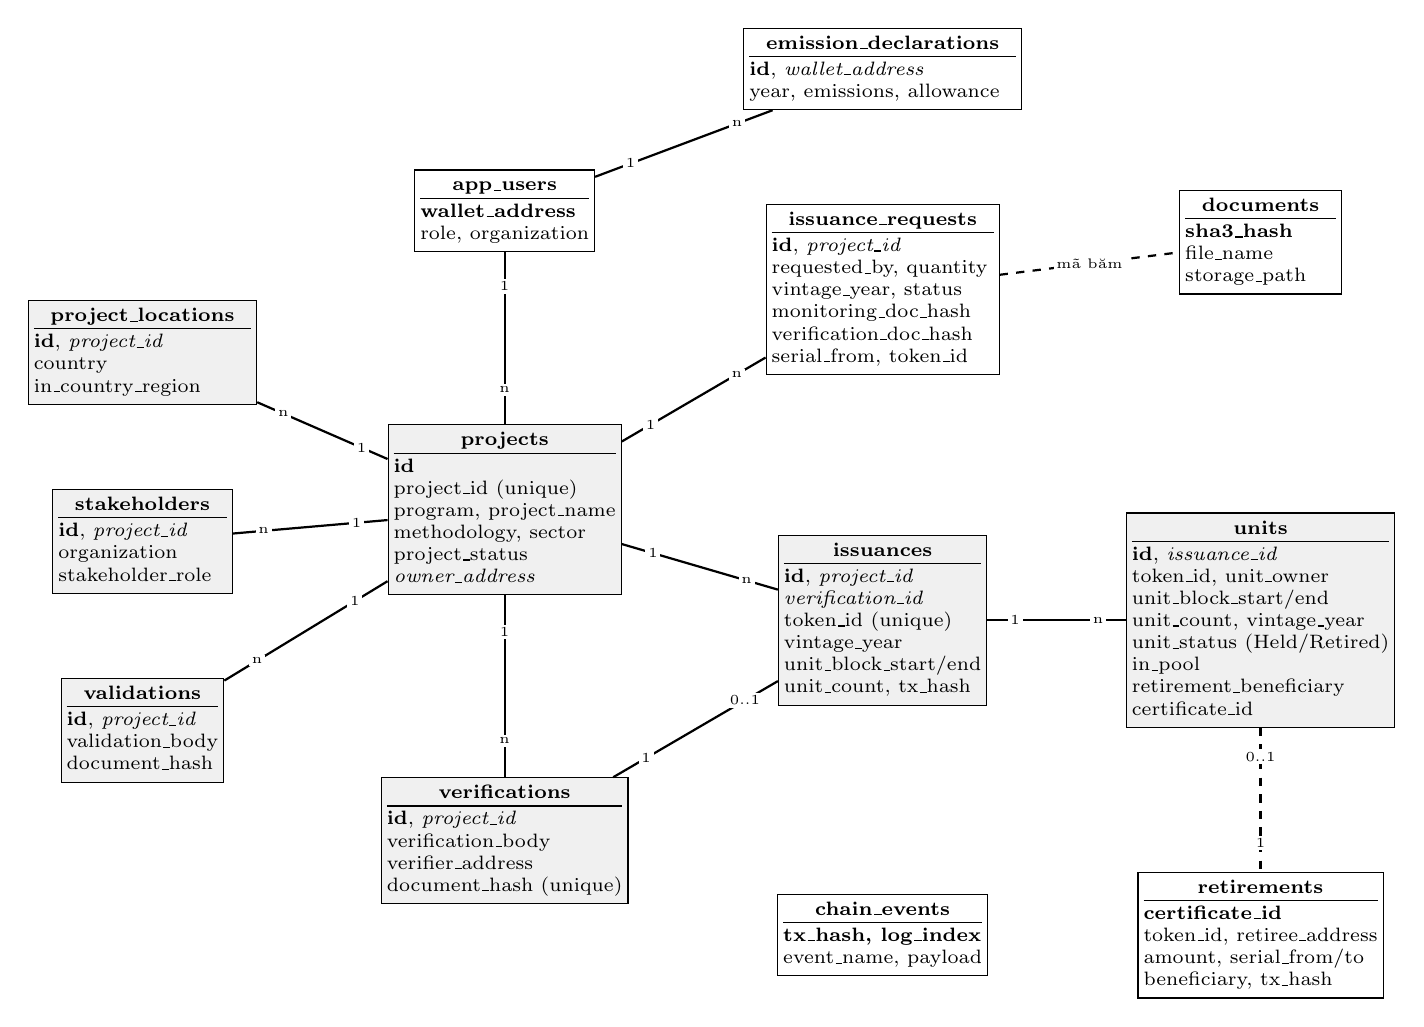
\begin{tikzpicture}[font=\scriptsize,
    bang/.style={draw, fill=white, inner sep=2pt, align=left},
    cad/.style={bang, fill=gray!12},
    lk/.style={draw, thick},
    n/.style={font=\tiny, fill=white, inner sep=1pt}]
  % Nhóm CAD Trust (nền xám)
  \node[cad] (proj) at (0,0) {\bangERD{projects}{%
     \textbf{id}\\ project\_id (unique)\\ program, project\_name\\ methodology, sector\\
     project\_status\\ \textit{owner\_address}}};
  \node[cad] (loc) at (-4.6,2.0) {\bangERD{project\_locations}{\textbf{id}, \textit{project\_id}\\ country\\ in\_country\_region}};
  \node[cad] (sh)  at (-4.6,-0.4) {\bangERD{stakeholders}{\textbf{id}, \textit{project\_id}\\ organization\\ stakeholder\_role}};
  \node[cad] (val) at (-4.6,-2.8) {\bangERD{validations}{\textbf{id}, \textit{project\_id}\\ validation\_body\\ document\_hash}};
  \node[cad] (ver) at (0,-4.2) {\bangERD{verifications}{\textbf{id}, \textit{project\_id}\\ verification\_body\\ verifier\_address\\ document\_hash (unique)}};
  \node[cad] (iss) at (4.8,-1.4) {\bangERD{issuances}{\textbf{id}, \textit{project\_id}\\ \textit{verification\_id}\\ token\_id (unique)\\ vintage\_year\\ unit\_block\_start/end\\ unit\_count, tx\_hash}};
  \node[cad] (unit) at (9.6,-1.4) {\bangERD{units}{\textbf{id}, \textit{issuance\_id}\\ token\_id, unit\_owner\\ unit\_block\_start/end\\ unit\_count, vintage\_year\\ unit\_status (Held/Retired)\\ in\_pool\\ retirement\_beneficiary\\ certificate\_id}};
  % Nhóm riêng của ứng dụng (nền trắng)
  \node[bang] (user) at (0,3.8) {\bangERD{app\_users}{\textbf{wallet\_address}\\ role, organization}};
  \node[bang] (req)  at (4.8,2.8) {\bangERD{issuance\_requests}{\textbf{id}, \textit{project\_id}\\ requested\_by, quantity\\ vintage\_year, status\\ monitoring\_doc\_hash\\ verification\_doc\_hash\\ serial\_from, token\_id}};
  \node[bang] (doc)  at (9.6,3.4) {\bangERD{documents}{\textbf{sha3\_hash}\\ file\_name\\ storage\_path}};
  \node[bang] (ret)  at (9.6,-5.4) {\bangERD{retirements}{\textbf{certificate\_id}\\ token\_id, retiree\_address\\ amount, serial\_from/to\\ beneficiary, tx\_hash}};
  \node[bang] (emi)  at (4.8,5.6) {\bangERD{emission\_declarations}{\textbf{id}, \textit{wallet\_address}\\ year, emissions, allowance}};
  \node[bang] (evt)  at (4.8,-5.4) {\bangERD{chain\_events}{\textbf{tx\_hash, log\_index}\\ event\_name, payload}};

  \draw[lk] (proj) -- node[n, pos=0.2]{1} node[n, pos=0.8]{n} (loc);
  \draw[lk] (proj) -- node[n, pos=0.2]{1} node[n, pos=0.8]{n} (sh);
  \draw[lk] (proj) -- node[n, pos=0.2]{1} node[n, pos=0.8]{n} (val);
  \draw[lk] (proj) -- node[n, pos=0.2]{1} node[n, pos=0.8]{n} (ver);
  \draw[lk] (proj) -- node[n, pos=0.2]{1} node[n, pos=0.8]{n} (iss);
  \draw[lk] (ver) -- node[n, pos=0.2]{1} node[n, pos=0.8]{0..1} (iss);
  \draw[lk] (iss) -- node[n, pos=0.2]{1} node[n, pos=0.8]{n} (unit);
  \draw[lk] (user) -- node[n, pos=0.2]{1} node[n, pos=0.8]{n} (proj);
  \draw[lk] (proj) -- node[n, pos=0.2]{1} node[n, pos=0.8]{n} (req);
  \draw[lk] (user) -- node[n, pos=0.2]{1} node[n, pos=0.8]{n} (emi);
  \draw[lk, dashed] (unit) -- node[n, pos=0.2]{0..1} node[n, pos=0.8]{1} (ret);
  \draw[lk, dashed] (req) -- node[n]{mã băm} (doc);
\end{tikzpicture}
\end{adjustbox}
\caption[Lược đồ cơ sở dữ liệu off-chain (nền xám: các bảng theo mô hình CAD Trust V2.0)]{Lược đồ cơ sở dữ liệu off-chain (nền xám: các bảng theo mô hình CAD Trust V2.0) \hinhtao[Claude]{21/10/2026}}
\label{fig:erd}
\end{figure}}

% ---------- Biểu đồ tuần tự ----------
% \dongdoi{tên nút}{x}{nhãn}{y cuối}: vẽ một đường đời (lifeline)
\newcommand{\dongdoi}[4]{%
  \node[draw, fill=white, minimum width=1.9cm, minimum height=0.7cm, align=center, font=\scriptsize] (#1) at (#2,0) {#3};
  \draw[dashed, gray] (#1.south) -- (#2,#4);}
% \tinnhan[kiểu mũi tên]{x1}{x2}{y}{nhãn}
\newcommand{\tinnhan}[5][->]{%
  \draw[#1, >=Stealth] (#2,#4) -- node[above, font=\scriptsize, align=center] {#5} (#3,#4);}

\newcommand{\HinhTuanTuMint}{%
\begin{figure}[htbp]
\centering
\begin{adjustbox}{max width=\textwidth}
\begin{tikzpicture}[yscale=1.2]
  % Sửa ngày 07/11/2026: VVB chỉ phê duyệt; cơ quan quản lý ký giao dịch phát hành (mint).
  \dongdoi{cda}{0}{Chủ dự án\\(trình duyệt)}{-12.0}
  \dongdoi{be}{3.8}{Backend API}{-12.0}
  \dongdoi{db}{6.6}{PostgreSQL}{-12.0}
  \dongdoi{vvb}{9.4}{VVB\\(trình duyệt)}{-12.0}
  \dongdoi{cq}{12.4}{Cơ quan quản lý\\(MetaMask)}{-12.0}
  \dongdoi{sc}{15.4}{CarbonCreditNFT}{-12.0}
  \dongdoi{ix}{18.4}{Bộ đồng bộ\\sự kiện}{-12.0}
  \tinnhan{0}{3.8}{-1.2}{POST /documents (báo cáo giám sát)}
  \tinnhan[<-]{0}{3.8}{-1.8}{sha3\_hash}
  \tinnhan{0}{3.8}{-2.5}{POST /issuance-requests}
  \tinnhan{3.8}{6.6}{-3.0}{INSERT, status = SUBMITTED}
  \tinnhan[<-]{3.8}{9.4}{-3.8}{GET /issuance-requests (danh sách chờ)}
  \tinnhan[<-]{3.8}{9.4}{-4.5}{POST /documents (báo cáo thẩm định)}
  \tinnhan[<-]{3.8}{9.4}{-5.2}{POST /issuance-requests/:id/approve}
  \tinnhan{3.8}{6.6}{-6.1}{kiểm tra mã băm chưa dùng;\\ INSERT verifications; APPROVED}
  \tinnhan[<-]{3.8}{12.4}{-6.9}{GET /issuance-requests (đã phê duyệt)}
  \tinnhan{3.8}{12.4}{-7.8}{tham số mint (to, projectId, vintage,\\ serialFrom, quantity, documentHash, uri)}
  \tinnhan{12.4}{15.4}{-8.5}{mintBatch(...) ký bằng ví\\ cơ quan quản lý}
  \node[draw, fill=white, font=\scriptsize, align=left, anchor=west] at (15.55,-9.2) {kiểm tra ISSUER\_ROLE,\\ sê-ri không chồng lấn,\\ documentHash chưa dùng};
  \tinnhan{15.4}{18.4}{-10.3}{sự kiện CreditMinted, Transfer}
  \draw[->, >=Stealth] (18.4,-10.9) -- node[above, font=\scriptsize, align=center, pos=0.3] {INSERT issuances, units (Held); yêu cầu $\rightarrow$ MINTED} (6.6,-10.9);
  \tinnhan[<-]{0}{3.8}{-11.5}{trạng thái MINTED, lô \#tokenId}
\end{tikzpicture}
\end{adjustbox}
\caption[Biểu đồ tuần tự quy trình yêu cầu cấp, thẩm định và phát hành tín chỉ]{Biểu đồ tuần tự quy trình yêu cầu cấp, thẩm định và phát hành tín chỉ \hinhtao[Claude]{21/10/2026; Updated: 07/11/2026}}
\label{fig:tuantu-mint}
\end{figure}}

\newcommand{\HinhTuanTuRetire}{%
\begin{figure}[htbp]
\centering
\begin{adjustbox}{max width=\textwidth}
\begin{tikzpicture}[yscale=1.2]
  \dongdoi{cda}{0}{Chủ dự án\\(MetaMask)}{-9.4}
  \dongdoi{dn}{3.4}{Doanh nghiệp\\(MetaMask)}{-9.4}
  \dongdoi{pool}{7.0}{CarbonPool\\(ERC-20)}{-9.4}
  \dongdoi{nft}{10.6}{CarbonCreditNFT\\(ERC-721)}{-9.4}
  \dongdoi{ix}{14.2}{Bộ đồng bộ\\+ CSDL}{-9.4}
  \tinnhan{0}{10.6}{-1.2}{safeTransferFrom(chủ dự án, pool, tokenId)}
  \tinnhan[<-]{7.0}{10.6}{-1.9}{onERC721Received(from, tokenId)}
  \node[draw, fill=white, font=\scriptsize, align=left, anchor=east] at (6.85,-2.6) {\_mint(from, remainingOf(tokenId));\\ NFT bị khóa trong pool};
  \tinnhan{0}{7.0}{-3.6}{transfer(doanh nghiệp, 300): bán từng phần}
  \tinnhan{3.4}{7.0}{-4.5}{retire(tokenId, 300, ...)}
  \node[draw, fill=white, font=\scriptsize, align=left, anchor=east] at (6.85,-5.1) {\_burn(doanh nghiệp, 300)};
  \tinnhan{7.0}{10.6}{-5.8}{retireFor(doanh nghiệp, tokenId, 300, ...)}
  \node[draw, fill=white, font=\scriptsize, align=left, anchor=west] at (10.75,-6.6) {retired += 300; lưu chứng nhận\\ (sê-ri, người hủy, thụ hưởng);\\ hủy hết thì \_burn(tokenId)};
  \tinnhan{10.6}{14.2}{-7.9}{sự kiện CreditRetired, Transfer}
  \tinnhan[<-]{3.4}{14.2}{-8.6}{GET /api/retirements/:id: chứng nhận hủy công khai}
\end{tikzpicture}
\end{adjustbox}
\caption[Biểu đồ tuần tự giao dịch qua pool và hủy tín chỉ]{Biểu đồ tuần tự giao dịch qua pool và hủy tín chỉ \hinhtao[Claude]{21/10/2026}}
\label{fig:tuantu-retire}
\end{figure}}

% ---------- Bảng API ----------
\newcommand{\BangAPI}{%
\begingroup\small
\renewcommand{\arraystretch}{1.15}
\begin{longtable}{|p{1.35cm}|>{\footnotesize}p{5.6cm}|>{\footnotesize\raggedright\arraybackslash}p{2.3cm}|>{\raggedright\arraybackslash}p{3.9cm}|}
\caption{Các endpoint của API REST}\label{tab:api}\\
\hline
\textbf{HTTP} & \textbf{Đường dẫn} & \textbf{Quyền} & \textbf{Chức năng}\\ \hline
\endfirsthead
\hline
\textbf{HTTP} & \textbf{Đường dẫn} & \textbf{Quyền} & \textbf{Chức năng}\\ \hline
\endhead
POST & /api/auth/nonce & Công khai & Lấy thông điệp đăng nhập cần ký\\ \hline
POST & /api/auth/login & Công khai & Xác minh chữ ký ví, cấp JWT; tạo tài khoản lần đầu\\ \hline
GET & /api/auth/me & Đã đăng nhập & Thông tin tài khoản\\ \hline
GET & /api/users & ADMIN & Danh sách tài khoản\\ \hline
PATCH & /api/users/:address/role & ADMIN & Đổi vai trò\\ \hline
GET & /api/projects & Công khai & Danh sách dự án kèm tổng đã cấp, đã hủy\\ \hline
GET & /api/projects/:id & Công khai & Chi tiết dự án, vị trí, các bên, thẩm định, đợt cấp\\ \hline
POST & /api/projects & PROJECT\_\allowbreak OWNER & Đăng ký dự án\\ \hline
PATCH & /api/projects/:id & Chủ dự án, ADMIN & Sửa thông tin; ADMIN đổi trạng thái\\ \hline
POST & /api/documents & Đã đăng nhập & Tải hồ sơ, trả mã băm keccak256\\ \hline
GET & /api/documents/:hash & Công khai & Thông tin, tải hồ sơ để đối chiếu mã băm\\ \hline
POST & /api/issuance-requests & PROJECT\_\allowbreak OWNER & Gửi yêu cầu cấp tín chỉ\\ \hline
GET & /api/issuance-requests[/:id] & Chủ dự án, VVB, ADMIN & Xem yêu cầu (kèm tham số mint nếu đã duyệt)\\ \hline
POST & /api/issuance-requests/:id/approve & VERIFIER & Phê duyệt, ghi thẩm định, trả tham số mint\\ \hline
POST & /api/issuance-requests/:id/reject & VERIFIER & Từ chối kèm lý do\\ \hline
GET & /api/issuances & Công khai & Danh sách đợt cấp\\ \hline
GET & /api/units & Công khai & Khối tín chỉ, lọc theo chủ sở hữu, trạng thái, lô, pool\\ \hline
GET & /api/units/lookup & Công khai & Tra cứu một số sê-ri\\ \hline
GET & /api/retirements[/:id] & Công khai & Danh sách, chi tiết chứng nhận hủy\\ \hline
GET & /api/metadata/requests/:id & Công khai & Metadata ERC-721 của lô\\ \hline
GET & /api/stats & Công khai & Số liệu tổng hợp\\ \hline
GET & /api/dashboard/me, /api/dashboard/:address & Đã đăng nhập; công khai & So sánh tín chỉ đã hủy với phát thải vượt hạn ngạch\\ \hline
PUT & /api/dashboard/emissions & Đã đăng nhập & Khai báo phát thải, hạn ngạch theo năm\\ \hline
GET & /api/cadtrust/projects/:id & Công khai & Xuất dữ liệu dự án theo cấu trúc CAD Trust\\ \hline
\end{longtable}
\endgroup}


Chương này trình bày thiết kế của hệ thống dựa trên các use case và yêu cầu phi chức năng ở Chương~\ref{chap:phantich}. Mục~\ref{sec:tk-kientruc} chọn kiến trúc lai kết hợp với kiến trúc phân lớp, rồi chia hệ thống thành các gói của ba thành phần frontend, backend và smart contract. Mục~\ref{sec:tk-chitiet} đi vào thiết kế chi tiết gồm giao diện, các lớp của hai smart contract và vòng đời của một lô tín chỉ, các biểu đồ trình tự cho hai quy trình chính, thiết kế API và thiết kế cơ sở dữ liệu. Trong mỗi phần, thiết kế ghi rõ ràng buộc chống tính toán kép nào nằm ở smart contract và ràng buộc nào chỉ nằm ở backend.

% ------------------------------------------------------------
\section{Thiết kế kiến trúc}
\label{sec:tk-kientruc}

\subsection*{Lựa chọn kiến trúc phần mềm}
\label{sec:kientruc}

Từ các yêu cầu ở Chương~\ref{chap:phantich}, đồ án chọn kiến trúc lai (hybrid architecture)\index{Kien truc lai@Kiến trúc lai (Hybrid Architecture)} kết hợp hai phần on-chain và off-chain, tổ chức theo kiến trúc phân lớp (layered architecture)\index{Kien truc phan lop@Kiến trúc phân lớp (Layered Architecture)} gồm bốn lớp (\autoref{fig:kientruc}). Phần off-chain giữ những dữ liệu có dung lượng lớn hoặc thay đổi thường xuyên như hồ sơ dự án, metadata và tài khoản người dùng, nhờ đó hệ thống giảm được chi phí lưu trữ và truy vấn nhanh hơn. Phần on-chain chỉ thực hiện ba thao tác mà bên thứ ba cần kiểm tra công khai là phát hành, chuyển nhượng và hủy tín chỉ. Mỗi lớp chỉ gọi tới lớp ngay bên dưới, nên có thể thay đổi một lớp, chẳng hạn chuyển nơi lưu tệp từ ổ đĩa cục bộ sang IPFS, mà không phải sửa smart contract đã triển khai.

Lớp thứ nhất là lớp nguồn dữ liệu và MRV (data source and MRV layer), cung cấp dữ liệu đầu vào cho việc cấp tín chỉ gồm hồ sơ thiết kế dự án (PDD), báo cáo giám sát và báo cáo thẩm định. Trong phạm vi đồ án, chủ dự án nhập thông tin và tải hồ sơ lên qua giao diện web, VVB tải lên báo cáo thẩm định, còn số liệu giám sát là dữ liệu mô phỏng. Đồ án không cài đặt việc thu thập dữ liệu tự động bằng cảm biến IoT theo mô hình của Vaccargiu và cộng sự~\cite{vaccargiu2026blockchain}, nhưng kiến trúc để sẵn điểm tích hợp để thiết bị gửi dữ liệu tổng hợp vào lớp thứ hai qua API RESTful.

Lớp thứ hai là lớp dịch vụ và lưu trữ off-chain (off-chain service and storage layer). Backend Node.js và Express cung cấp API RESTful\index{REST API}, xác thực người dùng và kiểm tra hồ sơ trước khi chuyển cho VVB. Cơ sở dữ liệu PostgreSQL\index{PostgreSQL} dựa trên các thực thể của mô hình CAD Trust V2.0 (Bảng~\ref{tab:cadtrust}) là Project, Stakeholders, Validations, Verifications, Issuances và Units~\cite{cadtrust2025datamodel}, còn tài khoản đăng nhập và phân quyền của ứng dụng nằm ở các bảng riêng. Hệ thống chỉ lưu đường dẫn và mã băm của tệp hồ sơ trong cơ sở dữ liệu. Một tiến trình đồng bộ sự kiện (event listener) đọc các sự kiện mà smart contract phát ra để cập nhật cơ sở dữ liệu; như vậy quyền sở hữu và trạng thái hủy lấy dữ liệu on-chain làm gốc, còn cơ sở dữ liệu off-chain chỉ là bản sao phục vụ truy vấn, giống vai trò của PostgreSQL trong hệ thống của UNDP~\cite{undp2024nationalregistry}.

Lớp thứ ba là lớp smart contract (on-chain smart contract layer), gồm hai smart contract viết bằng Solidity, dùng thư viện OpenZeppelin và triển khai trên testnet Sepolia. Sau khi VVB phê duyệt kết quả thẩm định, cơ quan quản lý ký giao dịch phát hành từ ví của mình, và hợp đồng NFT kiểm tra vai trò phát hành của bên gọi rồi tạo một token ERC-721\index{ERC-721} cho mỗi lô tín chỉ, lưu số lượng tCO$_2$e, dãy số sê-ri, mã băm hồ sơ và URI metadata, đồng thời từ chối dãy sê-ri trùng hoặc hồ sơ đã dùng. Hợp đồng không tự đánh giá nội dung hồ sơ, nên độ chính xác của số liệu vẫn dựa vào kết quả thẩm định của VVB. Hợp đồng pool nhận NFT, khóa NFT lại và trả cho người nạp lượng token ERC-20\index{ERC-20} tương ứng (1 token = 1 tCO$_2$e) để giao dịch từng phần; người giữ token có thể đổi token lấy lại một lô (redeem). Khi người dùng hủy tín chỉ, hàm hủy đốt token và ghi số lượng, dãy sê-ri, người thụ hưởng, nên phần tín chỉ này không thể chuyển nhượng hay hủy lại trong hệ thống. Chương Giải pháp và đóng góp sẽ phân tích chi tiết cơ chế này và giới hạn của nó.
% [VIẾT SAU] Khi \input Chap5 (giải pháp): đổi "Chương Giải pháp và đóng góp" thành "Chương~\ref{chap:giaiphap}".

Lớp thứ tư là lớp giao diện và API (presentation and API layer). Ứng dụng web Next.js dùng ethers.js kết nối ví MetaMask để người dùng tự ký các giao dịch phát hành, nạp pool, chuyển nhượng và hủy, nên khóa riêng không rời khỏi ví. Dashboard hiển thị tín chỉ đang nắm giữ, tín chỉ đã hủy và lịch sử giao dịch, đồng thời so sánh lượng tín chỉ doanh nghiệp đã hủy với lượng phát thải mà doanh nghiệp khai báo; người xem công khai tra cứu được tín chỉ theo số sê-ri kèm liên kết tới giao dịch trên Etherscan. API liên thông xuất dữ liệu dự án và tín chỉ theo cấu trúc CAD Trust V2.0 để trao đổi với hệ thống bên ngoài~\cite{cadtrust2025datamodel}, còn việc xuất báo cáo AEF như hệ thống của UNDP~\cite{undp2024nationalregistry} là hướng mở rộng.

\HinhKienTruc

\subsection*{Thiết kế tổng quan}
\label{subsec:tk-tongquan}

Từ kiến trúc bốn lớp, mã nguồn của hệ thống chia thành ba thành phần độc lập là frontend, backend và smart contract, mỗi thành phần gồm một số gói như \autoref{fig:goi}. Frontend chỉ phụ thuộc vào hai thành phần còn lại qua hai giao thức: gói lib gọi API REST của backend bằng HTTP và JSON, đồng thời gửi giao dịch tới smart contract qua JSON-RPC mà MetaMask cung cấp. Đây là điểm khác của một ứng dụng phi tập trung so với ứng dụng web ba tầng thông thường, vì giao dịch ghi on-chain đi thẳng từ ví của người dùng tới blockchain và không đi qua backend. Backend vì vậy không phụ thuộc vào frontend và cũng không gửi giao dịch nào; backend chỉ đọc sự kiện từ blockchain qua gói indexer. Trong thành phần smart contract, hợp đồng CarbonPool phụ thuộc vào CarbonCreditNFT để chuyển NFT và gọi hàm hủy, còn cả hai hợp đồng kế thừa các hợp đồng chuẩn của OpenZeppelin~\cite{openzeppelin2024contracts}. Không có phụ thuộc nào đi ngược từ tầng dưới lên tầng trên, nên đồ án có thể thay frontend hoặc viết lại backend mà không phải triển khai lại smart contract.

\HinhGoi

\subsection*{Thiết kế chi tiết gói}
\label{subsec:tk-chitietgoi}

Trong frontend, gói app chứa chín màn hình theo cơ chế định tuyến theo thư mục của Next.js, gói components chứa các thành phần dùng chung, còn gói lib gom toàn bộ phần giao tiếp với bên ngoài. Thành phần WalletProvider giữ trạng thái đăng nhập và địa chỉ ví cho mọi màn hình, còn Nav hiển thị các mục điều hướng theo vai trò của người dùng. Tệp chain.js tạo đối tượng hợp đồng từ ABI và địa chỉ triển khai trong contracts.json, kiểm tra MetaMask đang ở đúng mạng trước khi ký, và đổi tên lỗi revert thành thông báo dễ đọc; tệp api.js gắn JWT vào mỗi yêu cầu gửi tới backend. Nhờ cách gom này, các màn hình không gọi trực tiếp ethers.js hay fetch, nên khi địa chỉ hợp đồng hoặc địa chỉ backend thay đổi thì chỉ cần sửa gói lib.

Trong backend, gói routes gồm tám router Express tương ứng với tám nhóm chức năng, mỗi router nhận đối tượng truy cập cơ sở dữ liệu qua tham số khi khởi tạo, nên phần kiểm thử có thể thay PostgreSQL bằng một cơ sở dữ liệu trong bộ nhớ. Gói core gồm phần xác thực và phân quyền (auth.js), phần kiểm tra dữ liệu đầu vào (validate.js) và các lỗi HTTP chuẩn (errors.js). Gói indexer chạy độc lập với các router: tiến trình này định kỳ đọc các sự kiện CreditMinted, Transfer và CreditRetired theo từng đoạn khối, ghi vào cơ sở dữ liệu trong một giao dịch, rồi lưu số khối đã đồng bộ. Trong thành phần smart contract, hai hợp đồng tách theo trách nhiệm: CarbonCreditNFT giữ dữ liệu lô và chứng nhận hủy, còn CarbonPool chỉ giữ token có thể thay thế và danh sách NFT đang khóa. Thiết kế lớp của hai hợp đồng này nằm ở mục~\ref{sec:tk-chitiet}.

% ------------------------------------------------------------
\section{Thiết kế chi tiết}
\label{sec:tk-chitiet}

\subsection*{Thiết kế giao diện}
\label{subsec:tk-giaodien}
% [VIẾT SAU] Mẫu SoICT yêu cầu mockup cho 2–3 chức năng quan trọng (thẩm định và phát hành, ví tín chỉ, tra cứu)
% và ghi độ phân giải màn hình mục tiêu. Sinh viên tự vẽ mockup (Figma hoặc giấy) rồi chèn vào đây.

Giao diện của hệ thống gồm chín màn hình, chia thành nhóm công khai và nhóm cần đăng nhập (\autoref{tab:manhinh}). Mỗi màn hình phục vụ một hoặc vài use case ở Chương~\ref{chap:phantich}, và thanh điều hướng chỉ hiện những màn hình mà vai trò của người dùng có quyền dùng. Người dùng mới chọn vai trò chủ dự án hoặc doanh nghiệp mua rồi bấm ``Kết nối MetaMask''; hệ thống tạo tài khoản ở lần đăng nhập đầu, còn vai trò VVB và cơ quan quản lý chỉ do cơ quan quản lý cấp ở màn hình quản trị.

\begin{table}[!htbp]
    \centering
    \caption{Các màn hình của ứng dụng web}
    \label{tab:manhinh}
    \small
    \begin{tabularx}{\textwidth}{|L{2.6cm}|L{2.8cm}|L{2.6cm}|Y|}
        \hline
        \HD{Màn hình} & \HD{Đường dẫn} & \HD{Vai trò} & \HD{Chức năng chính} \\
        \hline
        Danh sách dự án & / & Công khai & Danh sách dự án kèm tổng số tín chỉ đã cấp, đã hủy \\
        \hline
        Chi tiết dự án & /projects/[id] & Công khai & Thông tin dự án, các bên, kết quả thẩm định, đợt cấp, tải hồ sơ \\
        \hline
        Tra cứu & /lookup & Công khai & Tra cứu theo mã dự án, vintage và số sê-ri (UC11) \\
        \hline
        Chứng nhận hủy & /certificates/[id] & Công khai & Chứng nhận hủy kèm liên kết giao dịch trên Etherscan \\
        \hline
        Dự án của tôi & /owner & Chủ dự án & Đăng ký dự án, gửi yêu cầu cấp, theo dõi trạng thái (UC05, UC06) \\
        \hline
        Thẩm định & /verifier & VVB & Xem yêu cầu, tải báo cáo thẩm định, phê duyệt hoặc từ chối (UC01) \\
        \hline
        Ví tín chỉ & /wallet & Đã đăng nhập & Lô đang giữ, nạp pool, chuyển token PCC, đổi lại lô, hủy tín chỉ, chứng nhận của tôi (UC07--UC09) \\
        \hline
        Dashboard & /dashboard & Đã đăng nhập & Khai báo phát thải, hạn ngạch theo năm và so sánh với tín chỉ đã hủy (UC10) \\
        \hline
        Quản trị & /admin & Cơ quan quản lý & Phát hành lô, quản lý tài khoản và vai trò, tạm dừng hợp đồng, đổi trạng thái dự án (UC02, UC03) \\
        \hline
    \end{tabularx}
\end{table}

Thiết kế giao diện tuân theo ba quy ước chung để người dùng chưa quen với ví blockchain vẫn thao tác được. Thứ nhất, mọi thao tác ghi on-chain dùng chung một thành phần nút: khi người dùng bấm, nút chuyển sang trạng thái ``Đang xử lý'' cho tới khi giao dịch có xác nhận, sau đó hiển thị kết quả kèm liên kết ``xem giao dịch'' trên Etherscan, hoặc hiển thị lỗi. Thứ hai, giao diện không hiển thị lỗi thô của thư viện mà đổi sang câu dễ hiểu, chẳng hạn người dùng từ chối ký thì hiện ``Bạn đã từ chối giao dịch trong MetaMask'', còn smart contract revert thì hiện tên lỗi như SerialOverlap hay ExceedsRemaining. Thứ ba, trạng thái của yêu cầu cấp và của khối tín chỉ hiển thị bằng nhãn màu theo đúng tên trạng thái trong cơ sở dữ liệu (SUBMITTED, APPROVED, REJECTED, MINTED, Held, Retired), để người dùng và người kiểm tra đối chiếu được với dữ liệu gốc.
% [CẦN SỬA MÃ] Theo thiết kế, nút phát hành nằm ở màn hình Quản trị (cơ quan quản lý); mã nguồn hiện đặt ở /verifier.

\subsection*{Thiết kế lớp}
\label{subsec:tk-lop}
\label{sec:tk-hopdong}

Phần quan trọng nhất của thiết kế lớp là hai smart contract, vì đây là nơi các ràng buộc chống tính toán kép có hiệu lực, và \autoref{fig:lophopdong} trình bày thuộc tính, phương thức và quan hệ kế thừa của hai hợp đồng này. Hợp đồng CarbonCreditNFT kế thừa ERC721URIStorage để mỗi lô là một NFT có URI metadata riêng~\cite{eip721}, kế thừa AccessControl để quản lý vai trò và Pausable để tạm dừng khi có sự cố. Dữ liệu của mỗi lô nằm trong cấu trúc CreditBatch gồm mã dự án, vintage, sê-ri đầu, số lượng, số đã hủy, mã băm báo cáo thẩm định, ví đã phát hành và thời điểm phát hành. Hai ánh xạ nextAvailableSerial và documentUsed giữ trạng thái chống phát hành kép: ánh xạ thứ nhất lưu sê-ri nhỏ nhất còn được phép cấp cho mỗi khóa keccak256(mã dự án, vintage), còn ánh xạ thứ hai đánh dấu mã băm báo cáo thẩm định đã dùng. Hàm mintBatch chỉ chấp nhận sê-ri đầu không nhỏ hơn giá trị trong nextAvailableSerial, nên hai lô của cùng dự án và vintage không thể có dãy sê-ri chồng lấn.

Hàm retire và retireFor cùng gọi một hàm nội bộ để hủy tín chỉ, và hàm này luôn hủy từ đầu phần sê-ri còn lại của lô: nếu một lô có sê-ri 1 đến 1.000 và đã hủy 300 thì lần hủy tiếp theo bắt đầu từ sê-ri 301. Mỗi lần hủy tạo một cấu trúc RetirementCertificate ghi dãy sê-ri, số lượng, người hủy, người thụ hưởng, lý do và thời điểm, rồi phát sự kiện CreditRetired; khi số đã hủy bằng số lượng của lô, hợp đồng đốt NFT để lô không thể chuyển nhượng nữa. Hàm retireFor chỉ dành cho hợp đồng có vai trò RETIREMENT\_AGENT\_ROLE và đang sở hữu NFT, tức là chỉ CarbonPool gọi được. Hợp đồng ghi đè hàm \_update của ERC-721 để chặn mọi lần chuyển NFT khi đang tạm dừng. Dữ liệu lô vẫn đọc được qua getBatch sau khi NFT đã bị đốt, nên lịch sử của một lô đã hủy hết không mất đi.

Hợp đồng CarbonPool kế thừa ERC20 với số chữ số thập phân bằng không, nghĩa là 1 token PCC luôn bằng đúng 1~tCO$_2$e và không chia nhỏ hơn~\cite{eip20}. Pool thực thi giao diện IERC721Receiver: mọi đường nạp NFT đều đi qua hàm onERC721Received, hàm này kiểm tra NFT đến từ đúng hợp đồng CarbonCreditNFT rồi đúc cho người nạp số token bằng phần còn lại của lô. Hàm redeem đốt số token bằng phần còn lại của lô và trả NFT về cho người gọi, còn hàm retire của pool đốt token trước rồi mới gọi retireFor. Nhờ vậy pool luôn giữ một bất biến: tổng cung token PCC bằng tổng phần còn lại của các lô đang khóa trong pool, và một lô không thể vừa bán dưới dạng NFT vừa bán dưới dạng token. Pool kế thừa ReentrancyGuard cho ba hàm deposit, redeem và retire, vì cả ba hàm đều gọi sang hợp đồng NFT, và lần gọi chuyển NFT có thể kích hoạt mã của bên nhận.
% [CẦN SỬA MÃ] Hình fig:lophopdong vẽ ISSUER_ROLE và trường issuer theo thiết kế; mã hiện là VERIFIER_ROLE và verifier.

\HinhLopHopDong

Vòng đời của một lô tín chỉ (\autoref{fig:trangthai}) gắn các trạng thái nghiệp vụ với các hàm của hai hợp đồng. Ba trạng thái đầu là Nháp, Chờ thẩm định và Bị từ chối chỉ tồn tại off-chain, ứng với các trạng thái của yêu cầu cấp trong cơ sở dữ liệu. Lô chuyển sang trạng thái Đã cấp khi hàm mintBatch thành công, và ở trạng thái này người giữ có thể chuyển nhượng NFT hoặc hủy một phần lô mà lô vẫn giữ nguyên trạng thái. Khi người giữ nạp lô vào pool, lô chuyển sang trạng thái Trong pool; ở trạng thái này token PCC lưu thông tự do và người giữ token có thể hủy một phần lô qua pool, còn hàm redeem đưa lô trở lại trạng thái Đã cấp. Lô kết thúc vòng đời ở trạng thái Đã hủy khi phần còn lại bằng không, dù lần hủy cuối diễn ra trực tiếp hay qua pool, và từ trạng thái này không có chuyển trạng thái nào khác.

\HinhTrangThai

\FloatBarrier
\subsection*{Biểu đồ trình tự}
\label{sec:tk-tuantu}

\autoref{fig:tuantu-mint} trình bày trình tự của quy trình yêu cầu cấp, thẩm định và phát hành, tức là luồng chính của ba use case UC06, UC01 và UC02. Chủ dự án tải báo cáo giám sát lên và nhận lại mã băm, sau đó gửi yêu cầu cấp; VVB tải báo cáo thẩm định lên và phê duyệt, còn backend kiểm tra mã băm chưa dùng, ghi bản ghi thẩm định và chuyển yêu cầu sang APPROVED. Cơ quan quản lý lấy tham số phát hành từ backend rồi ký giao dịch mintBatch bằng ví của mình, và hợp đồng tự kiểm tra lại vai trò, dãy sê-ri và mã băm. Cơ sở dữ liệu chỉ ghi đợt cấp và khối tín chỉ sau khi bộ đồng bộ đọc được sự kiện CreditMinted, nên trạng thái MINTED trong cơ sở dữ liệu luôn có một giao dịch on-chain tương ứng.

\HinhTuanTuMint

\autoref{fig:tuantu-retire} trình bày trình tự giao dịch qua pool và hủy tín chỉ. Chủ dự án chuyển NFT vào pool bằng safeTransferFrom, hợp đồng NFT gọi lại onERC721Received của pool, và pool đúc token cho chủ dự án theo phần còn lại của lô. Chủ dự án bán một phần token cho doanh nghiệp bằng hàm transfer chuẩn của ERC-20, sau đó doanh nghiệp gọi retire của pool, pool đốt token của doanh nghiệp rồi gọi retireFor để hợp đồng NFT ghi chứng nhận hủy với dãy sê-ri cụ thể. Bộ đồng bộ đọc sự kiện CreditRetired và cập nhật cơ sở dữ liệu, còn doanh nghiệp lấy chứng nhận hủy công khai qua API để gửi cho khách hàng hoặc cơ quan quản lý.

\HinhTuanTuRetire

\FloatBarrier
\subsection*{Thiết kế API}
\label{subsec:tk-api}

Backend cung cấp API REST với các endpoint ở \autoref{tab:api}, chia thành ba mức quyền: công khai, đã đăng nhập và theo vai trò. Mọi endpoint đọc dữ liệu tín chỉ, đợt cấp, chứng nhận hủy và hồ sơ đều công khai, vì yêu cầu kiểm tra độc lập ở mục~\ref{sec:phichucnang} đòi hỏi bên thứ ba truy cập được mà không cần tài khoản. Các endpoint ghi dữ liệu nghiệp vụ off-chain như đăng ký dự án, gửi yêu cầu cấp, phê duyệt hay từ chối yêu cầu yêu cầu đúng vai trò, và backend kiểm tra vai trò bằng một middleware chung trước khi vào xử lý. API không có endpoint nào gửi giao dịch on-chain: endpoint phê duyệt chỉ trả về tham số phát hành, còn việc ký giao dịch thuộc về ví của người dùng.

\BangAPI

Hệ thống xác thực người dùng bằng chữ ký ví thay cho mật khẩu, theo bốn bước. Frontend gửi địa chỉ ví tới endpoint nonce, và backend tạo một chuỗi ngẫu nhiên, lưu theo địa chỉ ví và trả về thông điệp đăng nhập chứa địa chỉ ví và chuỗi đó. Người dùng ký thông điệp bằng MetaMask theo phương thức personal\_sign, và frontend gửi chữ ký tới endpoint login. Backend khôi phục địa chỉ từ chữ ký bằng hàm verifyMessage của ethers.js~\cite{ethers2024docs} và so với địa chỉ đã khai; nếu khớp, backend cấp một JWT có hiệu lực tám giờ chứa địa chỉ ví và vai trò. Cách làm này có hai lợi ích: hệ thống không lưu mật khẩu nào, và tài khoản off-chain luôn gắn với đúng ví đã ký các giao dịch on-chain.

\FloatBarrier
\subsection*{Thiết kế cơ sở dữ liệu}
\label{subsec:tk-csdl}
\label{sec:tk-csdl}
\label{sec:onoffchain}

Trước khi thiết kế cơ sở dữ liệu, đồ án xác định dữ liệu nào nằm on-chain và dữ liệu nào nằm off-chain (\autoref{fig:onoffchain}, \autoref{tab:onoffchain}), theo các tiêu chí của Xu và cộng sự về chi phí, khả năng kiểm tra và tính riêng tư khi đặt dữ liệu lên blockchain~\cite{xu2017taxonomy}. Dữ liệu nằm on-chain là dữ liệu mà bên thứ ba cần kiểm tra và không ai được sửa, gồm quyền sở hữu, dữ liệu lô và chứng nhận hủy. Dữ liệu nằm off-chain là dữ liệu có dung lượng lớn, cần sửa trong quá trình xử lý hoặc cần bảo mật. Hai phía giữ nhất quán bằng hai cơ chế: mã băm của báo cáo thẩm định nằm trong dữ liệu lô on-chain, nên ai cũng kiểm tra được tệp off-chain có bị thay hay không, còn bộ đồng bộ sự kiện đảm bảo các bảng bản sao off-chain luôn đi sau dữ liệu on-chain chứ không tự tạo ra trạng thái mới.

\HinhOnOffChain

\begin{table}[!htbp]
    \centering
    \caption{Phân bổ dữ liệu giữa on-chain và off-chain}
    \label{tab:onoffchain}
    \small
    \begin{tabularx}{\textwidth}{|L{4.6cm}|L{2.6cm}|Y|}
        \hline
        \HD{Dữ liệu} & \HD{Nơi lưu} & \HD{Lý do} \\
        \hline
        Quyền sở hữu lô (NFT), số dư token PCC & On-chain & Bên thứ ba cần kiểm tra; là dữ liệu gốc khi hai phía lệch nhau \\
        \hline
        Dữ liệu lô: mã dự án, vintage, dãy sê-ri, số lượng, số đã hủy, mã băm báo cáo thẩm định & On-chain & Smart contract cần các giá trị này để chặn phát hành kép và gắn hồ sơ với lô \\
        \hline
        Chứng nhận hủy & On-chain & Bằng chứng hủy công khai, không ai sửa hay xóa được \\
        \hline
        Thông tin dự án theo CAD Trust V2.0 & Off-chain & Nhiều trường, cần sửa khi dự án thay đổi, phục vụ xuất dữ liệu liên thông \\
        \hline
        Tệp hồ sơ (PDD, báo cáo giám sát, báo cáo thẩm định) & Off-chain (kho tệp) & Dung lượng lớn; chỉ mã băm cần nằm on-chain \\
        \hline
        Tài khoản, vai trò off-chain, yêu cầu cấp, kết quả thẩm định & Off-chain & Quy trình còn có thể quay lại; thông tin định danh cần bảo mật \\
        \hline
        Khai báo phát thải, hạn ngạch & Off-chain & Dữ liệu riêng của doanh nghiệp, chỉ dùng cho dashboard \\
        \hline
        Bản sao đợt cấp, khối tín chỉ, chứng nhận hủy & Off-chain (đồng bộ) & Truy vấn nhanh theo dự án, chủ sở hữu, số sê-ri; on-chain vẫn là gốc \\
        \hline
    \end{tabularx}
\end{table}

\autoref{fig:erd} trình bày lược đồ cơ sở dữ liệu off-chain gồm mười lăm bảng chia thành hai nhóm. Nhóm thứ nhất (nền xám) gồm bảy bảng theo các thực thể của CAD Trust V2.0 là projects, project\_locations, stakeholders, validations, verifications, issuances và units~\cite{cadtrust2025datamodel}, với tên cột đặt theo tên trường của mô hình, ví dụ trường unitBlockStart thành cột unit\_block\_start. Nhóm thứ hai gồm tám bảng riêng của ứng dụng phục vụ đăng nhập (app\_users, auth\_nonces), quy trình nghiệp vụ (documents, issuance\_requests, retirements, emission\_declarations) và đồng bộ on-chain (chain\_events, sync\_state). Một dự án có nhiều đợt thẩm định và nhiều đợt cấp, mỗi đợt cấp ứng với đúng một NFT và có nhiều khối tín chỉ. Khi người dùng hủy một phần lô, bộ đồng bộ tách khối tín chỉ thành một dòng trạng thái Retired cho dãy sê-ri đã hủy và một dòng trạng thái Held cho phần còn lại, còn NFT on-chain vẫn giữ nguyên lô và chỉ tăng số đã hủy. Cách tách này giữ được ý nghĩa của bảng Units trong CAD Trust, nơi mỗi dòng là một khối sê-ri liên tục có cùng trạng thái.

\HinhERD

Lược đồ dùng ràng buộc của PostgreSQL để lặp lại các ràng buộc nghiệp vụ ở phía off-chain, nhờ đó backend phát hiện sai sót sớm trước khi người dùng tốn phí gas. Cột project\_id của bảng projects là duy nhất, tương ứng với mã dự án trên hệ thống đăng ký gốc; cột document\_hash của bảng verifications và của bảng issuances cũng là duy nhất, lặp lại ràng buộc documentUsed của smart contract; còn cột token\_id của bảng issuances là duy nhất vì mỗi đợt cấp ứng với một NFT. Cột trạng thái của yêu cầu cấp và của khối tín chỉ dùng ràng buộc CHECK để chỉ nhận các giá trị đã định nghĩa. Bảng chain\_events có khóa chính là cặp (tx\_hash, log\_index), nên khi bộ đồng bộ đọc lại một đoạn khối đã xử lý thì sự kiện trùng bị bỏ qua và cơ sở dữ liệu không ghi hai lần. Thiết kế hiện tại chưa xử lý trường hợp tổ chức lại chuỗi (reorg), vì bộ đồng bộ coi mọi khối đã đọc là cuối cùng; giới hạn này chấp nhận được trên testnet nhưng cần bổ sung khi triển khai thật.

% ------------------------------------------------------------
% Kết chương (Normal, không tiêu đề).
Qua chương này, tác giả đã thiết kế hệ thống theo kiến trúc lai bốn lớp, chia thành ba thành phần frontend, backend và smart contract với các phụ thuộc một chiều, trong đó giao dịch on-chain đi thẳng từ ví người dùng tới blockchain và backend không giữ khóa riêng nào. Thiết kế lớp của hai smart contract cho thấy ba ràng buộc chống tính toán kép trong phạm vi hệ thống đều có cơ chế kỹ thuật cụ thể: dãy sê-ri tăng dần và mã băm dùng một lần chặn phát hành kép, khóa NFT trong pool và bất biến tổng cung chặn bán kép, còn chứng nhận hủy với dãy sê-ri cụ thể và việc đốt NFT chặn hủy lại. Thiết kế cơ sở dữ liệu theo CAD Trust V2.0 lặp lại các ràng buộc này ở phía off-chain để phát hiện sai sót sớm, nhưng vẫn lấy dữ liệu on-chain làm gốc. Chương tiếp theo sẽ trình bày công nghệ sử dụng, việc cài đặt các thiết kế này, kết quả kiểm thử và triển khai trên testnet Sepolia.
% [VIẾT SAU] Khi \input Chap4: đổi "Chương tiếp theo" thành "Chương~\ref{chap:xaydung}".
